%        File: formeln.tex
%     Created: Mo Aug 15 03:00  2005 C
% Last Change: Mo Aug 15 03:00  2005 C
%
%\documentclass[a4paper]{report}
%\usepackage{ngerman}
%\usepackage.pdffig}
%\begin{document}

\chapter {Leistungsbewertung}
\section{Kenngr"o"sen der Zeit}

\paragraph{Mittlere Operationszeit:}
\begin{center}
$T = \sum_{i=1..n} t_i * p_i $
\end{center}
{\footnotesize $t_i$ \ldots Operationszeit des $i$-ten Befehls\\
$p_i$ \ldots Relative H"aufigkeit des $i$-ten Befehls im Befehlssatz}\\
%\vfill

\paragraph{Mittlere Operationszeit: } {\textit{alternativer Ausdruck}}
\begin{center}
$T = CPI * T_C + S * T_S [s] $
\end{center}
{\footnotesize $CPI$ \ldots cycles per instruction\\
$T_C$ \ldots Taktzykluszeit\\
$S$ \ldots Speicherbedarf bei Durchschnittsbefehl $[bit]$\\
$T_S$ \ldots Speicherzugriffszeit [s/bit]}\\
%\vfill

\paragraph{Verweilzeit, Wartezeit, Bedienzeit}
{\textit{Warteschlangenmodell}}
\begin{center}
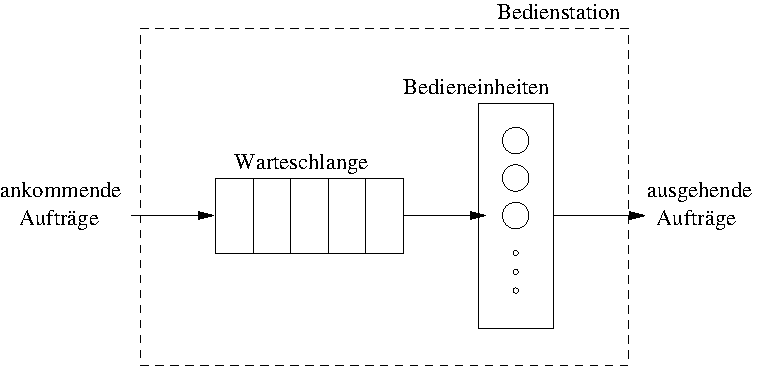
\includegraphics[width=10cm]{warteschlangenmodell.pdf}
\end{center}
{\footnotesize 
{\bf Bedienzeit }\ldots Dauer der Ausf"uhrung\\
{\bf Wartezeit }\ldots Dauer des Aufenthalts in der Warteschlange\\
{\bf Verweilzeit}\ldots Verz"ogerungszeit, Latenz, Antwortzeit}\\

\section {Kenngr"o"sen zum Durchsatz}
\paragraph{MIPS, MOPS, MFLOPS:}
MIPS/MOPS:  $\frac{1}{mittlere Operationszeit} = \frac{1}{T}$\\\\
\noindent
Da weder die Leistungsf"ahigkeit der einzelnen Operationen, noch die
relativen Geschwindigkeiten der beteiligten CPUs einberechnet werden
eignet sich dies nicht zum Vergleich von verschiedenen CPUs.
MFLOPS sind ebenfalls ung"unstig, da sie sich auf Programme beschr"anken,
die sehr Fliesskomma-zentriert sind. Auch die relative Komplexit"at
dieser Operationen wird nicht mit einbezogen.\\
\paragraph{Grenzdurchsatz, Verlustrate: } F"ur Warteschlangenmodell
relevant:\\\\
In Rechnernetzen spricht man beim \emph{Grenzdurchsatz} von der
\emph{Bandbreite}, wobei dies somit den maximalen Durchsatz darstellt. Da die
\emph{Latenz} in Netzen, die nahe der Grenzfrequenz operieren, oft sehr
hoch ist, ist als interessantes Ma"s die Anzahl der Auftr"age, die
eine bestimmte obere Grenze der Antwortzeit (Latenz) nicht
"uberschreiten von Interesse.
Die \emph{Verlustrate} hingegen beschreibt die Anzahl der
Einheiten, die pro Zeiteinheit verloren gehen.
\section{Auslastung}
Hierbei von Bedeutung ist das Verh"altnis von tats"achlich erreichtem
Durchsatz und Grenzdurchsatz. Dazu wird f"ur folgendes Beispiel der
\emph{Speed-Up}, also die Beschleunigung definiert: 
\begin{center}
$S_p(n)=\frac{T_1(n)}{T_p(n)}$
\end{center}
Es sei $T_p(n)$ die Laufzeit eines Algorithmus, der zur Ausf"uhrung
$p$ Prozessoren ben"otigt, bei einer Eingabe der L"ange $n$. Die
Berechnung der \emph{Effizienz} $E_p(n)$ berechnet sich nun aus dem
Verh"altnis des berechneten Speed-Ups $S_p(n)$ zu dem maximal
erreichbaren Speed-Up:
\begin{center}
$E_p(n)=\frac{S_p(n)}{p}$
\end{center}
Die maximal erreichbare Beschleunigung ist $p$-fach, da wir davon
ausgehen, dass das Problem sich durch die Verteilung auf $p$-Prozessoren
idealerweise um diesem Faktor beschleunigt. Damit gilt f"ur die Effizienz
folgende Ungleichung:
\begin{center}
$\frac{1}{p} \leq E_p(n) \leq 1$
\end{center}
Daher bezeichnet man einen parallelen Algorithmus mit $E_p(n)=1$ als
\emph{optimal}.

\section{Amdahls Gesetz}

Amdahls Gesetz besagt, dass die \emph{Leistungsverbesserung} durch den
Einsatz neuer Hardware abh"angig ist von
\begin{itemize}
\item dem Anteil an Ausf"uhrungszeit $r$, die ein Programm erbringt
und
\item der Beschleunigungsrate b, die durch die bessere Hardware erreicht
wird, wenn das \emph{gesamte} Programm getestet wird.
\end{itemize}
Mit anderen Worten besagt Amdahls Gesetz, dass sich der Aufwand f"ur die
Verbesserung nur dann lohne, wenn dadurch der h"aufig eintretende Fall
verbessere, also die neue Hardware h"aufig eingesetzt w"urde. 
\begin{center}
"`making the common case fast"'
\end{center}
Es ergibt sich also der Anteil an Ausf"uhrungszeit $r$, der sich
parallelisieren l"a"st und $(1-r)$, der Anteil f"ur den das nicht
klappt. Damit gilt f"ur die \emph{Gesamtausf"uhrungszeit} $T$:
\begin{center}
	$T = T * (1-r) + T * r$
\end{center}
\begin{center}
	$T_{verbessert} = T * (1-r) + \frac{T*r}{b}$\\
\end{center}
\begin{center}

$\rightarrow Speed-Up = \frac{T}{T_verbessert} = \frac{1}{(1-r) +
	\frac{r}{b}}$
\end{center}

\section{Methoden}
Viele Methoden zur Leistungsbewertung lassen sich in die drei Klassen
\emph{analytische Methoden, Messungen und Simulation} einordnen.
Analytische Methoden eignen sich gut zur schnellen Orientierung,
Simulationen sind dagegen sehr flexibel und Messungen liefern genaue
Aussagen.
\paragraph{Analytische Methoden. } Hierbei wird das Bewertungsproblem
auf der Grundlage von \emph{Gleichungen} approximativ oder numerisch gel"ost.
Diese Gleichungen sind mathematisch \emph{abgeschlossen} oder bestehen aus
Modellen. Sie werden abgeleitet aus z.Bsp. Warteschlangenmodellen,
Wartenetzen oder stochastischen Petrinetzen. Berechnet werden
quantitative Leistungsma"se wie \emph{Mittelwert, Durchsatz} oder
\emph{Latenz}. Das betroffene System wird dabei immer im \emph{station"aren
Zustand} betrachtet. Mit der Zunahme der Komplexit"at eines Systems wird
auch das Auffinden eines geeigneten analytischen Modells schwieriger
und aufwendiger.
\paragraph{Simulation. } Ohne das der zu bewertetende Rechner existieren
muss, wird eine Annahme "uber dessen Eigenschaften, also \emph{Struktur,
Betrieb, Betriebsprozesse}, getroffen und darauf ein \emph{Ablaufmodell}
gewonnen. Mit diesem Modell wird versucht genaue Leistungsaussagen "uber
den Rechner zu gewinnen. Simulationen sind \emph{Programme}, die
geschaffen werden, um das Verhalten eines Rechners auf einen anderen
abzubilden und werden meist in h"oheren Programmiersprachen, oder
Simulationssprachen geschrieben. Sehr h"aufig wird dabei eine
\emph{ereignisorientierte} Simulation (event driven simulation)
angewendet. Dabei wird die Zeit \emph{diskretisiert} und die Steuerung
wird durch bestimmte Ereignisse, wie z.Bsp. dem Ende einer
Auftragsbearbeitung ausgel"ost. Grunds"atzlich werden mit
\emph{deterministischen} und \emph{stochastischen} Simulationen zwei
Arten definiert, von denen es aber auch Mischformen gibt. Bei den
stochastischen Simulationen werden \emph{Zufallswerte} als Betriebsdaten
angenommen. Es ensteht hierbei das Problem der Generierung vern"unftiger
Zufallszahlen. Variablen sind w"ahrend des gesamten Simulationsprozesses
abrufbar und erlauben somit wesentlich aussagekr"aftigere Feststellungen
als dies bei analytischen Methoden m"oglich ist. Es lassen sich somit
beispielsweise \emph{einzelne Komponenten} einer Bewertung zuf"uhren.
Auf der anderen Seite stehen die deterministischen Simulationen. Mit
ihnen wird das \emph{funktionale} und \emph{Zeitverhalten} realer
Systeme genauer abgebildet als bei den stochastischen Simulationen. Der
Haupteinsatz dieser Simulation findet sich bei dem Entwurf neuer oder
der Optimierung bereits bestehender \emph{Funktionseinheiten} eines
bereits existierenden Systems. Detaillierte und deterministisch
arbeitende Modelle zu entwerfen ist hier m"oglich. Es wird hier weiterhin
unterschieden in die \emph{Trace-}gesteuerten und
\emph{ausf"uhrungsgesteuerten} Simulationen. Bei ersterem wird
beispielsweise das Verhalten von Speicherhierarchien simuliert. Mit
letzterem werden auf dem Simulationsmodell komplette Programme,
sogenannte \emph{Benchmark-}Programme, ausgef"uhrt und erlauben somit
eine noch realit"atsn"ahere Betrachtung.\\\\
Allgemein l"a"s sich f"ur Simulationen festhalten:
\begin{enumerate}
\item Simulationen bieten eine gute M"oglichkeit zum Entwurf von
Rechnern.
\item Sie erlauben eine Auswahl an Konfigurations"anderungen
vorzunehmen.
\item Mit der Zunahme der Komplexit"at steigen jedoch auch ihre Kosten.
\end{enumerate}
\paragraph{Messungen. } An existierenden System k"onnen zur
Leistungsfeststellung, also zum Erhalt von \emph{Leistungsma"szahlen},
Messungen durchgef"uhrt werden. Man nennt dies \emph{beobachtende
Leistungsbewertung}, deren Ziel es sein kann, entweder einzelne
Komponenten oder aber auch komplette Rechenanlagen zu vermessen. In
dieser Zielstellung steckt der Wunsch verschiedenene Rechenanlagen
\emph{vergleichen} zu k"onnen, theoretische Leistungsaussagen zu
\emph{validieren}, sowie den Betrieb \emph{"uberwachen} zu k"onnen.
Daher auch der Begriff "`beobachtende Leistungsbewertung"', im
Englischen \emph{monitoring}. Das monitoring kann \emph{ereignisbezogen}
und \emph{ereignisunabh"angig} sein. Es werden drei Typen von Messungen
unterschieden:
\begin {enumerate}
\item Monitoring
\item Benchmarking
\item Hybrides Monitoring
\end {enumerate}
Das Monitoring wird weiterhin unterschieden in \emph{Hardwaremonitoring}
und \emph{Softwaremonitoring}. Mit ersterem werden \emph{Messf"uhler} an
das Messobjekt angelegt und die Ergebnisse vom Hardwaremonitor
aufgesammelt. Vorteilhaft ist hier, dass die Messung den Ablauf des
Objektrechners nicht beinflu"st, hingegen muss mit einer gro"sen
Datenflut umgegangen werden. 

\begin{center}
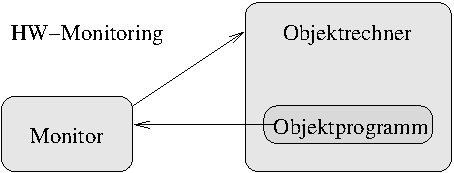
\includegraphics[height=2cm]{hw_monitor.pdf}
\end{center}

\noindent Hingegen wird beim Softwaremonitoring
die Messung durch das \emph{Objektprogramm} angesto"sen und durch ein
\emph{Messprogramm} dem Monitor zugef"uhrt. Vorteilhaft hier ist, dass
nur wenig Information "uber den Objektrechner notwendig ist und das die
Messprogramme auf vielen Rechnern laufen. Jedoch ist negativ zu
bemerken, dass durch den Eingriff in den Programmablauf das dynamische
Verhalten des Objektrechners verf"alscht wird.
\begin{center}
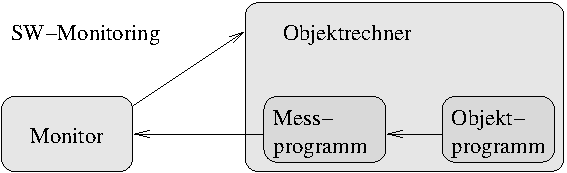
\includegraphics[height=2cm]{sw_monitor.pdf}
\end{center}
Eine spezielle Problemstellung stellt das Monitoring in verteilten
Systemen dar, in denen es keinen Masterrechner gibt, der die Daten �ber
die beteiligten Knoten zur Verf"ugung stellen kann. Daher werden 
\emph{Knotenmonitore} zur "Uberwachung von einzelnen Knoten oder
\emph{Verbindungsmonitore} zur "Uberwachung von Clustern von Rechnern
eingesetzt. Dabei stellt die \emph{unterschiedliche} Uhrzeit in den
beteiligten Rechnern das Hauptproblem dar, dass durch software- oder
hardwarem"assige Synchronisation, oder durch den Einsatz lokaler
Zeitstempel gel"ost werden kann.\\\\
Das Monitoring erf"ahrt seine Grenzen in der aus der zunehmenden
Integration resultierenden Schwierigkeit auf interne Signale zugreifen
zu k"onnen. Weiterhin wird durch \emph{virtuellen Speicher} eine
eindeutige Zuordnung zum Prozessor erschwert. Der Zugriff auf Daten-
oder Befehlscache wird verhindert. RISC-Prozessoren "andern die
Reihenfolge der Befehlsausf"uhrung und sorgen damit f"ur Probleme beim
Monitoring. Schliesslich kann die Steigerung der Taktraten zu einer
"uberm"a"sigen Datenflut f"uhren.\\\\

\noindent Unter dem Begriff {\bf Benchmarking} versteht man die
\emph{vergleichende Ausf"uhrung} ein und desselben (Mess-)programms auf
unterschiedlichen Rechnern. Der Rechner, der das Programm am schnellsten
ausf"uhrt ist demnach der schnellere Rechner. Hier liegt das Problem
begraben. In der Praxis ist es h"aufig vorgekommen, dass Compiler oder
Befehlss"atze manipuliert wurden, damit sie auf speziellen Benchmarks
bessere Leistung erzeugen. Benchmarks erm"oglichen es, zus"atzliche
Informationen "uber Compiler, Betriebssystem und auch die Genauigkeit
der Ergebnisse zu gewinnen. Es gibt vier Typen von Benchmarks:

\begin{enumerate}
\item Reale Programme (h"aufig verwendete Programme)
\item Kernels (kurze kritische Passagen aus realen Programmen)
\item Toy Benchmarks (kleine, einfache, schnell "ubertragbare Programme)
\item Synthetische Benchmarks (testen spezielle Instruktionen)
\end{enumerate}

\noindent Zu den synthetischen Benchmarks geh"oren die mittlerweile
veralteten Dhrystone und Wheatstone Benchmarks, der LINPACK-Benchmark
und die SPECint, sowie SPECfp-Benchmarks.


\chapter{Fehlertoleranz}

Rechnersysteme werden auch in sensiblen Bereichen eingesetzt, in denen
ein Ausfall oder Fehlfunktion eklatante Folgen haben k"onnen. Es wird daher
nach hoher Verl"asslichkeit gefragt. Die \emph{Fehlerintoleranz}
beschreibt Methoden zur \emph{Vermeidung} von Fehlverhalten. Die
\emph{Fehlertoleranz} versucht dagegen erw"unschtes Verhalten durch
ein System auch dann zu erhalten, wenn mit einer bestimmen Anzahl von
Fehlern gerechnet werden muss. Fehler lassen sich aufgrund verschiedener
Eigenschaften klassifizieren. So beschreibt die \emph{Dauer eines
Fehlers}, ob ein Fehler permanent oder nur vorr"ubergehend auftritt. Die
\emph{Auswirkung eines Fehlers} erkl"art, ob ein Fehler nur auf eine
Komponente wirkt ($\rightarrow$ Einfachfehler) oder ob eine Fehlerquelle
mehrere Fehler erzeugt ($\rightarrow$ Mehrfachfehler). Finde sich ein
\emph{Fehler im Lebenszyklus eines Rechners}, so besteht die Frage ob es
sich um einen Konstruktionsfehler (Entwurfs-, Implementierungs- oder
Herstellungsfehler) handelt oder ob es ein Betriebsfehler ist, also ob
er w"ahrend des Betriebs(Bedienungs- oder Wartungsfehler) auftritt. Ein
weiteres Klassifizierungsmerkmal ist der \emph{Ort des Fehlers}, also ob
er in der Hardware oder Software angesiedelt ist Ein weiteres
Klassifizierungsmerkmal ist der \emph{Ort des Fehlers}, also ob er in
der Hardware oder Software angesiedelt ist.\\\\
\section{Zuverl"assigkeit und Verf"ugbarkeit}
Zur Erfassung der Fehlertoleranz werden quantitative Gr"o"sen relevant.
Eine wichtige Gr"o"se ist die \emph{Zuverl"assigkeit} $R(t)$, die
bedingte Wahrscheinlichkeit, dass ein System das Zeitintervall $[0,t)$
"uberlebt. Es gilt:
\begin{center}
	$R(0)=1 \longrightarrow$ Das Ger"at ist zum Zeitpunkt 0 funktionst"uchtig.
\end{center}
\begin{center}
	$R(\infty)=0\longrightarrow$ Nach gen"ugend langer Zeit f"allt das Ger"at aus.
\end{center}
Eine weitere Gr"o"se ist die \emph{Ausfallrate} $\lambda(t)$, f"ur die
im nicht konstanten Fall gilt:
\begin{center}
$\lambda(t)=-\frac{\delta R(t)}{dt R(t)}$
\end{center}
Ist die Aufallrate $\lambda$ konstant, so gilt beispielsweise:
\begin{center}
$R(t)=e^{-\lambda t}$
\end{center}
Dieses Beispiel nutzen wir f"ur die Beschreibung einer weiteren Gr"o"se,
n"amlich der \emph{mittleren Funktionszeit} (mean team to failure):
\begin{center}
$MTF=\int_{i=0}^{\infty}R(t)dt= \frac{1}{\lambda}$
\end{center}
Mit der sogenannten Badewannenfunktion lassen sich Fr"uhausf"alle und
Sp"atausf"alle beschreiben. Eine andere wichtige Gr"o"se stellt die
\emph{Verf"ugbarkeit} dar. F"ur eine nicht-redundante Einheit mit
Ausfallrate $\lambda$ und Reparaturrate $\mu$ (Kehrwert der
Reparaturzeit $MTR$ gilt
\begin{center}
$A=\frac{MTF}{MTR+MTF}=\frac{\lambda}{\lambda + \mu}$
\end{center}

\begin{center}
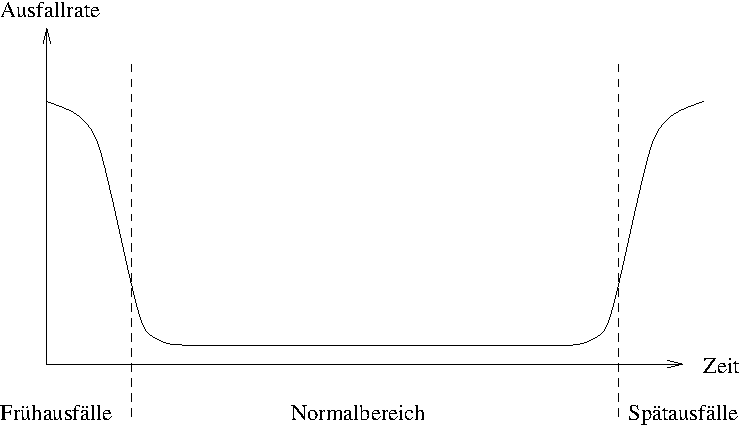
\includegraphics[height=5cm]{badewanne.pdf}
\end{center}

\noindent So lassen sich beispielsweise f"ur die Halbleiterproduktion
die Fr"uausf"alle durch die Technik des \emph{burn in} lokalisieren und
die entsprechend fehlerhaften Produkte entfernen, was die Lebensdauer
von bereitgestellten Halbleitern nat"urlich erh"oht. 

\section{Redundanztechniken}
Der Begriff \emph{Redundanz} beschreibt hier das Hinzuf"ugen von
Hardware oder Software in ein System um Fehlererkennung und
Reaktion darauf zu erm"oglichen. Die zentralen Begriffe sind hierf"ur
die \emph{Fehlerdiagnose} und \emph{Fehlerbehandlung}. Die
Fehlerdiagnose findet als \emph{Selbstest} im System im laufenden
Betrieb statt. Die Fehlerbehandlung setzt sich aus der
\emph{Rekonfiguration}, also der Isolierung der fehlerhaften Teile in HW
und SW und aus dem \emph{Wiederanlauf} zusammen. Beim Wiederanlauf wird
das System nach dem Ausschluss fehlerhafter Teile in der Grundzustand
versetzt. Ausserdem sollen \emph{Sicherungspunkte} angelegt werden, die
als sp"atere R"ucksetzpunkte dienen k"onnen.\\\\
Die Redundanz wird unterschieden in \emph{dynamische} und
\emph{statische} Redundanz. In der statischen Redundanz sind alle
Elemente, die f"ur die Fehlertoleranz notwendig sind, st"andig in
Betrieb, w"ahrend bei der dynamischen Redundanz notwendige Elemente
on-demand zugeschalten werden.
\section{Beispiele fehlertoleranter Systeme}
Hierzu gelten \emph{Universalrechnersysteme}, wie
transaktionsorientierte Datenbankanwendungen, die hohe Zuverl"assigkeit
erfordern. Es sind dabei alle funktionalen Komponenten, also
CPU/Speicher/Busse/Peripherie statisch und/oder dynamisch redundant.
Ebenso sind L"ufter- und Spannungsversorgung redundant. Als anderes
Beispiel seien \emph{eingebettete Rechnersysteme} genannt, bei denen
geringe Kosten und hohe Kompatibilit"at im Vordergrund stehen. Hierbei
wurden Mechanismen entwickelt, die den Austausch von Komponenten zur
Laufzeit erm"oglichen (hot-swap, hot-plugin). Dazu werden zumeist
Bussysteme verwendet, die dies unterst"utzenm wie USB. Ein letztes
Beispiel sei mit RAID genannt. RAID steht f"ur \emph{Redundant array of
inexpensive disks} und stellt ein Peripheriesystem dar. Der Grundgedanke
ist, dass mechanische Komponenten wie hier zum Beispiel Festplatten eine
sehr viel geringe MTF haben. Die MTF sinkt sogar noch weiter, wenn man
die Anzahl der Festplatten in einem System erh"oht. RAID bietet hierf"ur
eine L"osung. Drei Eigenschaften sind kennzeichnend:
\begin{enumerate}
\item Eine Menge \emph{physischer} Platten wird durch das Betriebssystem
als \emph{eine logische} Platte aufgefasst.
\item Die Datenspeicherung erfolgt verteilt.
\item Ausnutzen der Redundanz der verf"ugbaren Kapazit"aten um im
Fehlerfall die Wahrscheinlichkeit zur Wiederherstellung zu erh"ohen.
\end{enumerate}

\noindent Die Vorteile liegen auf der Hand. Es wird eine wesentlich h"ohere
Zuverl"assigkeit erm"oglicht und der parallele Zugriff auf die Platten
erh"oht die Leistungsf"ahigkeit der E/A. 

%\end{document}

